% Options for packages loaded elsewhere
\PassOptionsToPackage{unicode}{hyperref}
\PassOptionsToPackage{hyphens}{url}
%
\documentclass[
]{article}
\usepackage{amsmath,amssymb}
\usepackage{iftex}
\ifPDFTeX
  \usepackage[T1]{fontenc}
  \usepackage[utf8]{inputenc}
  \usepackage{textcomp} % provide euro and other symbols
\else % if luatex or xetex
  \usepackage{unicode-math} % this also loads fontspec
  \defaultfontfeatures{Scale=MatchLowercase}
  \defaultfontfeatures[\rmfamily]{Ligatures=TeX,Scale=1}
\fi
\usepackage{lmodern}
\ifPDFTeX\else
  % xetex/luatex font selection
\fi
% Use upquote if available, for straight quotes in verbatim environments
\IfFileExists{upquote.sty}{\usepackage{upquote}}{}
\IfFileExists{microtype.sty}{% use microtype if available
  \usepackage[]{microtype}
  \UseMicrotypeSet[protrusion]{basicmath} % disable protrusion for tt fonts
}{}
\makeatletter
\@ifundefined{KOMAClassName}{% if non-KOMA class
  \IfFileExists{parskip.sty}{%
    \usepackage{parskip}
  }{% else
    \setlength{\parindent}{0pt}
    \setlength{\parskip}{6pt plus 2pt minus 1pt}}
}{% if KOMA class
  \KOMAoptions{parskip=half}}
\makeatother
\usepackage{xcolor}
\usepackage[margin=1in]{geometry}
\usepackage{color}
\usepackage{fancyvrb}
\newcommand{\VerbBar}{|}
\newcommand{\VERB}{\Verb[commandchars=\\\{\}]}
\DefineVerbatimEnvironment{Highlighting}{Verbatim}{commandchars=\\\{\}}
% Add ',fontsize=\small' for more characters per line
\usepackage{framed}
\definecolor{shadecolor}{RGB}{248,248,248}
\newenvironment{Shaded}{\begin{snugshade}}{\end{snugshade}}
\newcommand{\AlertTok}[1]{\textcolor[rgb]{0.94,0.16,0.16}{#1}}
\newcommand{\AnnotationTok}[1]{\textcolor[rgb]{0.56,0.35,0.01}{\textbf{\textit{#1}}}}
\newcommand{\AttributeTok}[1]{\textcolor[rgb]{0.13,0.29,0.53}{#1}}
\newcommand{\BaseNTok}[1]{\textcolor[rgb]{0.00,0.00,0.81}{#1}}
\newcommand{\BuiltInTok}[1]{#1}
\newcommand{\CharTok}[1]{\textcolor[rgb]{0.31,0.60,0.02}{#1}}
\newcommand{\CommentTok}[1]{\textcolor[rgb]{0.56,0.35,0.01}{\textit{#1}}}
\newcommand{\CommentVarTok}[1]{\textcolor[rgb]{0.56,0.35,0.01}{\textbf{\textit{#1}}}}
\newcommand{\ConstantTok}[1]{\textcolor[rgb]{0.56,0.35,0.01}{#1}}
\newcommand{\ControlFlowTok}[1]{\textcolor[rgb]{0.13,0.29,0.53}{\textbf{#1}}}
\newcommand{\DataTypeTok}[1]{\textcolor[rgb]{0.13,0.29,0.53}{#1}}
\newcommand{\DecValTok}[1]{\textcolor[rgb]{0.00,0.00,0.81}{#1}}
\newcommand{\DocumentationTok}[1]{\textcolor[rgb]{0.56,0.35,0.01}{\textbf{\textit{#1}}}}
\newcommand{\ErrorTok}[1]{\textcolor[rgb]{0.64,0.00,0.00}{\textbf{#1}}}
\newcommand{\ExtensionTok}[1]{#1}
\newcommand{\FloatTok}[1]{\textcolor[rgb]{0.00,0.00,0.81}{#1}}
\newcommand{\FunctionTok}[1]{\textcolor[rgb]{0.13,0.29,0.53}{\textbf{#1}}}
\newcommand{\ImportTok}[1]{#1}
\newcommand{\InformationTok}[1]{\textcolor[rgb]{0.56,0.35,0.01}{\textbf{\textit{#1}}}}
\newcommand{\KeywordTok}[1]{\textcolor[rgb]{0.13,0.29,0.53}{\textbf{#1}}}
\newcommand{\NormalTok}[1]{#1}
\newcommand{\OperatorTok}[1]{\textcolor[rgb]{0.81,0.36,0.00}{\textbf{#1}}}
\newcommand{\OtherTok}[1]{\textcolor[rgb]{0.56,0.35,0.01}{#1}}
\newcommand{\PreprocessorTok}[1]{\textcolor[rgb]{0.56,0.35,0.01}{\textit{#1}}}
\newcommand{\RegionMarkerTok}[1]{#1}
\newcommand{\SpecialCharTok}[1]{\textcolor[rgb]{0.81,0.36,0.00}{\textbf{#1}}}
\newcommand{\SpecialStringTok}[1]{\textcolor[rgb]{0.31,0.60,0.02}{#1}}
\newcommand{\StringTok}[1]{\textcolor[rgb]{0.31,0.60,0.02}{#1}}
\newcommand{\VariableTok}[1]{\textcolor[rgb]{0.00,0.00,0.00}{#1}}
\newcommand{\VerbatimStringTok}[1]{\textcolor[rgb]{0.31,0.60,0.02}{#1}}
\newcommand{\WarningTok}[1]{\textcolor[rgb]{0.56,0.35,0.01}{\textbf{\textit{#1}}}}
\usepackage{graphicx}
\makeatletter
\def\maxwidth{\ifdim\Gin@nat@width>\linewidth\linewidth\else\Gin@nat@width\fi}
\def\maxheight{\ifdim\Gin@nat@height>\textheight\textheight\else\Gin@nat@height\fi}
\makeatother
% Scale images if necessary, so that they will not overflow the page
% margins by default, and it is still possible to overwrite the defaults
% using explicit options in \includegraphics[width, height, ...]{}
\setkeys{Gin}{width=\maxwidth,height=\maxheight,keepaspectratio}
% Set default figure placement to htbp
\makeatletter
\def\fps@figure{htbp}
\makeatother
\setlength{\emergencystretch}{3em} % prevent overfull lines
\providecommand{\tightlist}{%
  \setlength{\itemsep}{0pt}\setlength{\parskip}{0pt}}
\setcounter{secnumdepth}{-\maxdimen} % remove section numbering
\ifLuaTeX
  \usepackage{selnolig}  % disable illegal ligatures
\fi
\IfFileExists{bookmark.sty}{\usepackage{bookmark}}{\usepackage{hyperref}}
\IfFileExists{xurl.sty}{\usepackage{xurl}}{} % add URL line breaks if available
\urlstyle{same}
\hypersetup{
  pdftitle={General structure of a simulation study},
  pdfauthor={Ian Hussey},
  hidelinks,
  pdfcreator={LaTeX via pandoc}}

\title{General structure of a simulation study}
\usepackage{etoolbox}
\makeatletter
\providecommand{\subtitle}[1]{% add subtitle to \maketitle
  \apptocmd{\@title}{\par {\large #1 \par}}{}{}
}
\makeatother
\subtitle{Using the example of estimating the statistical power of
Student's independent \emph{t}-test}
\author{Ian Hussey}
\date{28 Februar, 2024}

\begin{document}
\maketitle

{
\setcounter{tocdepth}{2}
\tableofcontents
}
\hypertarget{overview-of-tutorial}{%
\section{Overview of tutorial}\label{overview-of-tutorial}}

This tutorial teaches you about the essential components of a simulation
study and the general steps involved in actually writing one. It does
this using the example of a simulation that answers a question that is
relevant to many social scientists:

\emph{The independent t-test assumes that participants are allocated
equally to two groups. How much does an unbalanced design lower the
statistical power of the test?}

We will somewhat gloss over some important details, e.g., the specifics
of how data is generated using pseudo random number generators, a more
fine-grained treatment of how we write functions, and diagnostics of
whether your simulation is performing well. We will return to these in
future lessons.

\hypertarget{essential-components-general-steps}{%
\section{Essential components \& general
steps}\label{essential-components-general-steps}}

The essential \emph{components} of a simulation are:

\begin{enumerate}
\def\labelenumi{\arabic{enumi}.}
\tightlist
\item
  Generate pseudo-random data set with known properties
\item
  Analyse data with a statistical method
\item
  Repeat 1 \& 2 many times (`iterations')
\item
  Collect and aggregate results across iterations
\item
  Make it an experiment: Systematically vary parameters in Step 1
  (between factor) and/or compare different ways to do Step 2 (within
  factor)
\end{enumerate}

However, the way you \emph{build} a simulation is much more iterative
than this final product. Each component must be both built and inspected
by itself, and then checked to make sure that the components work
together in the correct manner, like a fine Swiss watch.

The general steps for actually building one involve:

\begin{enumerate}
\def\labelenumi{\arabic{enumi}.}
\tightlist
\item
  Generate a \emph{single} pseudo-random data set with known properties,
  using hard-coded variables
\item
  Analyse this \emph{single} data set with a statistical method, using
  hard-coded variables
\item
  Convert the data generation code to a function, making it as abstract
  as necessary {[}Component 1{]}
\item
  Convert the data analysis code to a function, making it as abstract as
  necessary {[}Component 2{]}
\item
  Ensure that experiment parameters, data generation function, and data
  analysis code play together nicely (i.e., can pass values between one
  another in a workflow, and save values appropriately {[}Component
  4{]}). Do this using a small number of parameters and just one or two
  iterations.
\item
  Increase the number of iterations and parameters and actually run the
  simulation as a whole {[}Component 4 and 5{]}
\item
  Check the assumptions of the simulation have been adequately met
\item
  Interpret the results of the simulation
\end{enumerate}

This tutorial focuses on the general practical steps, but always keep
the essential components in mind as the guiding principles of why we're
doing something.

\hypertarget{generate-data-and-apply-and-analysis-once-using-hard-coded-arguments}{%
\section{\texorpdfstring{Generate data and apply and analysis
\emph{once} using hard coded
arguments}{Generate data and apply and analysis once using hard coded arguments}}\label{generate-data-and-apply-and-analysis-once-using-hard-coded-arguments}}

\hypertarget{generate-some-data-for-an-independent-t-test}{%
\subsection{Generate some data for an independent
t-test}\label{generate-some-data-for-an-independent-t-test}}

condition: factor with two levels (control, intervention) score: numeric
of normally distributed data (within each condition), with different
means, and SD = 1.

To sample data from a normally distributed population, we use the
pseudo-random number generator for normal data built into R:
\texttt{rnorm()}. Note that many packages exist to help you generate
different types of data more easily, including \{MASS\}, \{faux\},
\{simstudy\}, and \{lavaan\}. These can be very helpful, but here we'll
do it manually for the moment.

\begin{Shaded}
\begin{Highlighting}[]
\CommentTok{\# dependencies}
\FunctionTok{library}\NormalTok{(tidyr)}
\FunctionTok{library}\NormalTok{(dplyr)}
\end{Highlighting}
\end{Shaded}

\begin{verbatim}
## 
## Attache Paket: 'dplyr'
\end{verbatim}

\begin{verbatim}
## Die folgenden Objekte sind maskiert von 'package:stats':
## 
##     filter, lag
\end{verbatim}

\begin{verbatim}
## Die folgenden Objekte sind maskiert von 'package:base':
## 
##     intersect, setdiff, setequal, union
\end{verbatim}

\begin{Shaded}
\begin{Highlighting}[]
\FunctionTok{library}\NormalTok{(forcats)}
\FunctionTok{library}\NormalTok{(readr)}
\FunctionTok{library}\NormalTok{(purrr) }
\FunctionTok{library}\NormalTok{(ggplot2)}
\FunctionTok{library}\NormalTok{(effsize)}

\CommentTok{\# set the seed value for pseudo random number generators to make results reproducible  }
\FunctionTok{set.seed}\NormalTok{(}\DecValTok{42}\NormalTok{)}

\NormalTok{generated\_data }\OtherTok{\textless{}{-}} 
  \FunctionTok{bind\_rows}\NormalTok{(}
    \CommentTok{\# given that cohen\textquotesingle{}s d = (m2 {-} m1)/SD\_pooled, simply setting SDs to 1 and mean\_control to 0 lets us control the cohen\textquotesingle{}s d = mean\_intervention}
    \FunctionTok{tibble}\NormalTok{(}\AttributeTok{condition =} \StringTok{"control"}\NormalTok{,}
           \AttributeTok{score =} \FunctionTok{rnorm}\NormalTok{(}\AttributeTok{n =} \DecValTok{100}\NormalTok{, }\AttributeTok{mean =} \FloatTok{0.0}\NormalTok{, }\AttributeTok{sd =} \DecValTok{1}\NormalTok{)), }
    \FunctionTok{tibble}\NormalTok{(}\AttributeTok{condition =} \StringTok{"intervention"}\NormalTok{,}
           \AttributeTok{score =} \FunctionTok{rnorm}\NormalTok{(}\AttributeTok{n =} \DecValTok{100}\NormalTok{, }\AttributeTok{mean =} \FloatTok{0.5}\NormalTok{, }\AttributeTok{sd =} \DecValTok{1}\NormalTok{))}
\NormalTok{  )}

\FunctionTok{head}\NormalTok{(generated\_data)}
\end{Highlighting}
\end{Shaded}

\begin{verbatim}
## # A tibble: 6 x 2
##   condition  score
##   <chr>      <dbl>
## 1 control    1.37 
## 2 control   -0.565
## 3 control    0.363
## 4 control    0.633
## 5 control    0.404
## 6 control   -0.106
\end{verbatim}

\hypertarget{fit-a-students-independnet-t-test}{%
\subsection{\texorpdfstring{Fit a Student's independnet
\emph{t}-test}{Fit a Student's independnet t-test}}\label{fit-a-students-independnet-t-test}}

\begin{Shaded}
\begin{Highlighting}[]
\FunctionTok{t.test}\NormalTok{(}\AttributeTok{formula =}\NormalTok{ score }\SpecialCharTok{\textasciitilde{}}\NormalTok{ condition, }
       \AttributeTok{data =}\NormalTok{ generated\_data,}
       \AttributeTok{var.equal =} \ConstantTok{TRUE}\NormalTok{,}
       \AttributeTok{alternative =} \StringTok{"two.sided"}\NormalTok{)}
\end{Highlighting}
\end{Shaded}

\begin{verbatim}
## 
##  Two Sample t-test
## 
## data:  score by condition
## t = -2.7554, df = 198, p-value = 0.006409
## alternative hypothesis: true difference in means between group control and group intervention is not equal to 0
## 95 percent confidence interval:
##  -0.6519651 -0.1080379
## sample estimates:
##      mean in group control mean in group intervention 
##                 0.03251482                 0.41251629
\end{verbatim}

\hypertarget{create-a-data-generating-function}{%
\section{Create a data generating
function}\label{create-a-data-generating-function}}

\hypertarget{make-the-existing-code-more-abstract}{%
\subsection{Make the existing code more
abstract}\label{make-the-existing-code-more-abstract}}

Move the values to variables

\begin{Shaded}
\begin{Highlighting}[]
\CommentTok{\# parameters for simulated data}
\NormalTok{n\_control }\OtherTok{=} \DecValTok{50}
\NormalTok{n\_intervention }\OtherTok{=}\NormalTok{ n\_control}
\NormalTok{mean\_control }\OtherTok{=} \DecValTok{0}
\NormalTok{mean\_intervention }\OtherTok{=} \FloatTok{0.5}
\NormalTok{sd\_control }\OtherTok{=} \DecValTok{1}
\NormalTok{sd\_intervention }\OtherTok{=} \DecValTok{1}

\CommentTok{\# generate data using these parameters}
\NormalTok{generated\_data }\OtherTok{\textless{}{-}} 
  \FunctionTok{bind\_rows}\NormalTok{(}
    \FunctionTok{tibble}\NormalTok{(}\AttributeTok{condition =} \StringTok{"control"}\NormalTok{,}
           \AttributeTok{score =} \FunctionTok{rnorm}\NormalTok{(}\AttributeTok{n =}\NormalTok{ n\_control, }\AttributeTok{mean =}\NormalTok{ mean\_control, }\AttributeTok{sd =}\NormalTok{ sd\_control)),}
    \FunctionTok{tibble}\NormalTok{(}\AttributeTok{condition =} \StringTok{"intervention"}\NormalTok{,}
           \AttributeTok{score =} \FunctionTok{rnorm}\NormalTok{(}\AttributeTok{n =}\NormalTok{ n\_intervention, }\AttributeTok{mean =}\NormalTok{ mean\_intervention, }\AttributeTok{sd =}\NormalTok{ sd\_intervention))}
\NormalTok{  ) }

\CommentTok{\# view the generated data}
\FunctionTok{head}\NormalTok{(generated\_data)}
\end{Highlighting}
\end{Shaded}

\begin{verbatim}
## # A tibble: 6 x 2
##   condition  score
##   <chr>      <dbl>
## 1 control   -2.00 
## 2 control    0.334
## 3 control    1.17 
## 4 control    2.06 
## 5 control   -1.38 
## 6 control   -1.15
\end{verbatim}

\hypertarget{convert-this-to-a-function}{%
\subsection{Convert this to a
function}\label{convert-this-to-a-function}}

Abstracting code into functions is a learned skill. For the moment, see
if you can follow the logic of the function and where it came from in
the hard coded original version.

\begin{Shaded}
\begin{Highlighting}[]
\CommentTok{\# define function}
\NormalTok{generate\_data }\OtherTok{\textless{}{-}} \ControlFlowTok{function}\NormalTok{(n\_control, }\CommentTok{\# the parameters are now function arguments}
\NormalTok{                          n\_intervention,}
\NormalTok{                          mean\_control,}
\NormalTok{                          mean\_intervention,}
\NormalTok{                          sd\_control,}
\NormalTok{                          sd\_intervention) \{}
  
\NormalTok{  data }\OtherTok{\textless{}{-}} 
    \FunctionTok{bind\_rows}\NormalTok{(}
      \FunctionTok{tibble}\NormalTok{(}\AttributeTok{condition =} \StringTok{"control"}\NormalTok{,}
             \AttributeTok{score =} \FunctionTok{rnorm}\NormalTok{(}\AttributeTok{n =}\NormalTok{ n\_control, }\AttributeTok{mean =}\NormalTok{ mean\_control, }\AttributeTok{sd =}\NormalTok{ sd\_control)),}
      \FunctionTok{tibble}\NormalTok{(}\AttributeTok{condition =} \StringTok{"intervention"}\NormalTok{,}
             \AttributeTok{score =} \FunctionTok{rnorm}\NormalTok{(}\AttributeTok{n =}\NormalTok{ n\_intervention, }\AttributeTok{mean =}\NormalTok{ mean\_intervention, }\AttributeTok{sd =}\NormalTok{ sd\_intervention))}
\NormalTok{    ) }
  
  \FunctionTok{return}\NormalTok{(data)}
\NormalTok{\}}
  
\CommentTok{\# call the function with example arguments}
\NormalTok{generated\_data }\OtherTok{\textless{}{-}} \FunctionTok{generate\_data}\NormalTok{(}\AttributeTok{n\_control =} \DecValTok{50}\NormalTok{,}
                                \AttributeTok{n\_intervention =} \DecValTok{50}\NormalTok{,}
                                \AttributeTok{mean\_control =} \DecValTok{0}\NormalTok{,}
                                \AttributeTok{mean\_intervention =} \FloatTok{0.5}\NormalTok{,}
                                \AttributeTok{sd\_control =} \DecValTok{1}\NormalTok{,}
                                \AttributeTok{sd\_intervention =} \DecValTok{1}\NormalTok{)}

\CommentTok{\# view the generated data}
\FunctionTok{head}\NormalTok{(generated\_data)}
\end{Highlighting}
\end{Shaded}

\begin{verbatim}
## # A tibble: 6 x 2
##   condition    score
##   <chr>        <dbl>
## 1 control   -0.00462
## 2 control    0.760  
## 3 control    0.0390 
## 4 control    0.735  
## 5 control   -0.146  
## 6 control   -0.0579
\end{verbatim}

\hypertarget{check-the-data-is-what-you-meant-to-data}{%
\subsection{Check the data is what you meant to
data}\label{check-the-data-is-what-you-meant-to-data}}

In general, you should inspect the data thoroughly, check the data
types, plot it, conduct other sanity checks, etc. For the moment, we
apply just the most basic test: check that the analysis can be fit to
data generated by the data generation function. For the moment, the
specific results don't matter as much as whether it can accept the data.
That is, your data generation will have to be aligned with your data
analysis code (e.g., both make use of the variables score
{[}continuous{]} and condition {[}factor with two levels{]}).

\begin{Shaded}
\begin{Highlighting}[]
\FunctionTok{t.test}\NormalTok{(}\AttributeTok{formula =}\NormalTok{ score }\SpecialCharTok{\textasciitilde{}}\NormalTok{ condition, }
       \AttributeTok{data =}\NormalTok{ generated\_data, }\CommentTok{\# using the data generated in the previous chunk}
       \AttributeTok{var.equal =} \ConstantTok{TRUE}\NormalTok{,}
       \AttributeTok{alternative =} \StringTok{"two.sided"}\NormalTok{)}
\end{Highlighting}
\end{Shaded}

\begin{verbatim}
## 
##  Two Sample t-test
## 
## data:  score by condition
## t = -3.9348, df = 98, p-value = 0.0001557
## alternative hypothesis: true difference in means between group control and group intervention is not equal to 0
## 95 percent confidence interval:
##  -1.0364241 -0.3414872
## sample estimates:
##      mean in group control mean in group intervention 
##                -0.06154135                 0.62741428
\end{verbatim}

\hypertarget{create-a-data-analysis-function}{%
\section{Create a data analysis
function}\label{create-a-data-analysis-function}}

\hypertarget{make-the-existing-code-more-abstract-1}{%
\subsection{Make the existing code more
abstract}\label{make-the-existing-code-more-abstract-1}}

Now do the same abstraction for the analysis.

Rather than just printing all the results of the t test to the console,
extract the p value specifically as a column in a tibble. In general,
you usually want to extract the results of analyses in
\texttt{tidy\ data} format. Note that the \{parameters\} and \{broom\}
packages can be very helpful for doing this for you for many common
types of analysis, but here we're do it manually.

\begin{Shaded}
\begin{Highlighting}[]
\NormalTok{res\_t\_test }\OtherTok{\textless{}{-}} \FunctionTok{t.test}\NormalTok{(}\AttributeTok{formula =}\NormalTok{ score }\SpecialCharTok{\textasciitilde{}}\NormalTok{ condition, }
                     \AttributeTok{data =}\NormalTok{ generated\_data,}
                     \AttributeTok{var.equal =} \ConstantTok{TRUE}\NormalTok{,}
                     \AttributeTok{alternative =} \StringTok{"two.sided"}\NormalTok{)}

\NormalTok{res }\OtherTok{\textless{}{-}} \FunctionTok{tibble}\NormalTok{(}\AttributeTok{p =}\NormalTok{ res\_t\_test}\SpecialCharTok{$}\NormalTok{p.value)}

\NormalTok{res}
\end{Highlighting}
\end{Shaded}

\begin{verbatim}
## # A tibble: 1 x 1
##          p
##      <dbl>
## 1 0.000156
\end{verbatim}

\hypertarget{convert-this-to-a-function-1}{%
\subsection{Convert this to a
function}\label{convert-this-to-a-function-1}}

\begin{Shaded}
\begin{Highlighting}[]
\NormalTok{analyse\_data }\OtherTok{\textless{}{-}} \ControlFlowTok{function}\NormalTok{(data) \{}
  
\NormalTok{  res\_t\_test }\OtherTok{\textless{}{-}} \FunctionTok{t.test}\NormalTok{(}\AttributeTok{formula =}\NormalTok{ score }\SpecialCharTok{\textasciitilde{}}\NormalTok{ condition, }
                       \AttributeTok{data =}\NormalTok{ data,}
                       \AttributeTok{var.equal =} \ConstantTok{TRUE}\NormalTok{,}
                       \AttributeTok{alternative =} \StringTok{"two.sided"}\NormalTok{)}
  
\NormalTok{  res }\OtherTok{\textless{}{-}} \FunctionTok{tibble}\NormalTok{(}\AttributeTok{p =}\NormalTok{ res\_t\_test}\SpecialCharTok{$}\NormalTok{p.value)}
  
  \FunctionTok{return}\NormalTok{(res)}
\NormalTok{\}}
\end{Highlighting}
\end{Shaded}

\hypertarget{compare-original-hard-coded-version-with-functionalised-version}{%
\section{Compare original hard-coded version with functionalised
version}\label{compare-original-hard-coded-version-with-functionalised-version}}

\hypertarget{original-manual-code-copied-from-above}{%
\subsection{Original manual code, copied from
above}\label{original-manual-code-copied-from-above}}

\begin{Shaded}
\begin{Highlighting}[]
\FunctionTok{set.seed}\NormalTok{(}\DecValTok{42}\NormalTok{)}

\NormalTok{generated\_data }\OtherTok{\textless{}{-}} 
  \FunctionTok{bind\_rows}\NormalTok{(}
    \FunctionTok{tibble}\NormalTok{(}\AttributeTok{condition =} \StringTok{"control"}\NormalTok{,}
           \AttributeTok{score =} \FunctionTok{rnorm}\NormalTok{(}\AttributeTok{n =} \DecValTok{100}\NormalTok{, }\AttributeTok{mean =} \FloatTok{0.0}\NormalTok{, }\AttributeTok{sd =} \DecValTok{1}\NormalTok{)),}
    \FunctionTok{tibble}\NormalTok{(}\AttributeTok{condition =} \StringTok{"intervention"}\NormalTok{,}
           \AttributeTok{score =} \FunctionTok{rnorm}\NormalTok{(}\AttributeTok{n =} \DecValTok{100}\NormalTok{, }\AttributeTok{mean =} \FloatTok{0.5}\NormalTok{, }\AttributeTok{sd =} \DecValTok{1}\NormalTok{))}
\NormalTok{  ) }

\FunctionTok{t.test}\NormalTok{(}\AttributeTok{formula =}\NormalTok{ score }\SpecialCharTok{\textasciitilde{}}\NormalTok{ condition, }
       \AttributeTok{data =}\NormalTok{ generated\_data,}
       \AttributeTok{var.equal =} \ConstantTok{TRUE}\NormalTok{,}
       \AttributeTok{alternative =} \StringTok{"two.sided"}\NormalTok{)}
\end{Highlighting}
\end{Shaded}

\begin{verbatim}
## 
##  Two Sample t-test
## 
## data:  score by condition
## t = -2.7554, df = 198, p-value = 0.006409
## alternative hypothesis: true difference in means between group control and group intervention is not equal to 0
## 95 percent confidence interval:
##  -0.6519651 -0.1080379
## sample estimates:
##      mean in group control mean in group intervention 
##                 0.03251482                 0.41251629
\end{verbatim}

\hypertarget{new-code-using-functions-copied-from-above}{%
\subsection{New code using functions, copied from
above}\label{new-code-using-functions-copied-from-above}}

\begin{Shaded}
\begin{Highlighting}[]
\FunctionTok{set.seed}\NormalTok{(}\DecValTok{42}\NormalTok{)}

\NormalTok{generated\_data }\OtherTok{\textless{}{-}} \FunctionTok{generate\_data}\NormalTok{(}\AttributeTok{n\_control =} \DecValTok{50}\NormalTok{,}
                                \AttributeTok{n\_intervention =}\NormalTok{ n\_control,}
                                \AttributeTok{mean\_control =} \DecValTok{0}\NormalTok{,}
                                \AttributeTok{mean\_intervention =} \FloatTok{0.5}\NormalTok{,}
                                \AttributeTok{sd\_control =} \DecValTok{1}\NormalTok{,}
                                \AttributeTok{sd\_intervention =} \DecValTok{1}\NormalTok{)}

\NormalTok{results }\OtherTok{\textless{}{-}} \FunctionTok{analyse\_data}\NormalTok{(generated\_data)}

\NormalTok{results}
\end{Highlighting}
\end{Shaded}

\begin{verbatim}
## # A tibble: 1 x 1
##         p
##     <dbl>
## 1 0.00297
\end{verbatim}

\hypertarget{do-it-lots-of-times-and-summarize-across-them}{%
\section{Do it lots of times and summarize across
them}\label{do-it-lots-of-times-and-summarize-across-them}}

\begin{Shaded}
\begin{Highlighting}[]
\FunctionTok{set.seed}\NormalTok{(}\DecValTok{42}\NormalTok{)}

\CommentTok{\# define the number of iterations}
\NormalTok{iterations }\OtherTok{\textless{}{-}} \DecValTok{100}

\CommentTok{\# declare a vector to store each iteration\textquotesingle{}s results in}
\NormalTok{p\_values }\OtherTok{\textless{}{-}} \FunctionTok{numeric}\NormalTok{(iterations)}

\CommentTok{\# use for loop to repeat its content many times}
\CommentTok{\# for the \textquotesingle{}i\textquotesingle{}{-}th element of the series 1 to \textasciigrave{}iterations\textasciigrave{} (i.e., 1, 2, 3, ... iterations), run the following code:}
\ControlFlowTok{for}\NormalTok{(i }\ControlFlowTok{in} \DecValTok{1}\SpecialCharTok{:}\NormalTok{iterations)\{ }
  \CommentTok{\# generate data}
\NormalTok{  generated\_data }\OtherTok{\textless{}{-}} \FunctionTok{generate\_data}\NormalTok{(}\AttributeTok{n\_control =} \DecValTok{50}\NormalTok{,}
                                  \AttributeTok{n\_intervention =} \DecValTok{50}\NormalTok{,}
                                  \AttributeTok{mean\_control =} \DecValTok{0}\NormalTok{,}
                                  \AttributeTok{mean\_intervention =} \FloatTok{0.5}\NormalTok{,}
                                  \AttributeTok{sd\_control =} \DecValTok{1}\NormalTok{,}
                                  \AttributeTok{sd\_intervention =} \DecValTok{1}\NormalTok{)}
  
  \CommentTok{\# analyse data}
\NormalTok{  results }\OtherTok{\textless{}{-}} \FunctionTok{analyse\_data}\NormalTok{(generated\_data)}
  
  \CommentTok{\# store result of this iteration}
  \CommentTok{\# the i{-}th element of the iterations vector will be replaced with the p value of the current iteration\textquotesingle{}s t{-}test}
\NormalTok{  p\_values[i] }\OtherTok{\textless{}{-}}\NormalTok{ results}\SpecialCharTok{$}\NormalTok{p}
\NormalTok{\}}

\CommentTok{\# summarize individual analysis results across iterations to find stimulation results}
\FunctionTok{mean}\NormalTok{(p\_values }\SpecialCharTok{\textless{}}\NormalTok{ .}\DecValTok{05}\NormalTok{)}
\end{Highlighting}
\end{Shaded}

\begin{verbatim}
## [1] 0.77
\end{verbatim}

Congratulations, you've just run your first simulation. Let's remind
ourselves what it did.

\begin{itemize}
\tightlist
\item
  Data generating process (i.e., population effect): true effect Cohen's
  d = 0.50 (i.e., difference in means = 0.50, both SDs = 1), with 50
  participants per condition.
\item
  Data analysis: independent t-test p value.
\item
  Iterations: 100
\item
  Summary across iterations: For 50 participants per condition, when the
  true population effect exists (is non zero, i.e., Cohen's d = .50), an
  independent t-test produces statistically significant p values in 77\%
  of cases. This is the definition of statistical power: the proportion
  of cases where effects that do exist are detected (i.e., true-positive
  results).
\end{itemize}

\hypertarget{what-if-i-want-my-simulation-to-do-more-complex-things}{%
\section{What if I want my simulation to do more complex
things?}\label{what-if-i-want-my-simulation-to-do-more-complex-things}}

The above code isn't enough because we want our simulation to be an
experiment with multiple between-conditions. How might we accomplish
this?

We could extend the method above, but it gets tricky very quickly.

For example, if I wanted to see how changing the number of participants
in (a) the control condition and (b) the intervention condition so that
either can be anywhere between 50 and 250 (in steps of 50), including
having different number between them (e.g., control = 200, intervention
= 100), then I'll have to either:

\begin{itemize}
\tightlist
\item
  Repeat my code a lot. This is always a bad idea. Repeating simple
  tasks we're bad at doing ourselves is the reason we invented
  computers.
\item
  Abstract the code further in some way, such as using more for-loops.
\end{itemize}

Before you look at this code, know that it much harder to understand and
much harder to write too. I'm showing you this method so that you know
it exists and is the most basic way of doing it - not because we are
going to do it in any of the rest of this course.

\begin{Shaded}
\begin{Highlighting}[]
\FunctionTok{set.seed}\NormalTok{(}\DecValTok{42}\NormalTok{)}

\CommentTok{\# define the number of iterations}
\NormalTok{iterations }\OtherTok{\textless{}{-}} \DecValTok{100}
\NormalTok{n\_control\_conditions }\OtherTok{\textless{}{-}} \FunctionTok{seq}\NormalTok{(}\AttributeTok{from =} \DecValTok{50}\NormalTok{, }\AttributeTok{to =} \DecValTok{250}\NormalTok{, }\AttributeTok{by =} \DecValTok{50}\NormalTok{)}
\NormalTok{n\_intervention\_conditions }\OtherTok{\textless{}{-}} \FunctionTok{seq}\NormalTok{(}\AttributeTok{from =} \DecValTok{50}\NormalTok{, }\AttributeTok{to =} \DecValTok{250}\NormalTok{, }\AttributeTok{by =} \DecValTok{50}\NormalTok{)}

\CommentTok{\# initialize results list}
\NormalTok{simulation\_results }\OtherTok{\textless{}{-}} \FunctionTok{list}\NormalTok{()}

\CommentTok{\# counter for appending results}
\NormalTok{result\_counter }\OtherTok{\textless{}{-}} \DecValTok{1}

\CommentTok{\# use nested for loops to iterate over conditions}
\ControlFlowTok{for}\NormalTok{(k }\ControlFlowTok{in}\NormalTok{ n\_intervention\_conditions)\{ }\CommentTok{\# for each of the \textquotesingle{}k\textquotesingle{}{-}th members of the n\_intervention\_conditions vector ... }
  \ControlFlowTok{for}\NormalTok{(j }\ControlFlowTok{in}\NormalTok{ n\_control\_conditions)\{ }\CommentTok{\# ... and for each of the \textquotesingle{}j\textquotesingle{}{-}th members of the n\_control\_conditions vector ...}
    \ControlFlowTok{for}\NormalTok{(i }\ControlFlowTok{in} \DecValTok{1}\SpecialCharTok{:}\NormalTok{iterations)\{ }\CommentTok{\# ... and for each value of \textquotesingle{}i\textquotesingle{} in the sequence 1 to iterations, run the following code with those values of i, j, and k:}
      
      \CommentTok{\# generate data}
\NormalTok{      generated\_data }\OtherTok{\textless{}{-}} \FunctionTok{generate\_data}\NormalTok{(}\AttributeTok{n\_control =}\NormalTok{ j,  }\CommentTok{\# current value of j}
                                      \AttributeTok{n\_intervention =}\NormalTok{ k,  }\CommentTok{\# current value of k}
                                      \AttributeTok{mean\_control =} \DecValTok{0}\NormalTok{,}
                                      \AttributeTok{mean\_intervention =} \FloatTok{0.5}\NormalTok{,}
                                      \AttributeTok{sd\_control =} \DecValTok{1}\NormalTok{,}
                                      \AttributeTok{sd\_intervention =} \DecValTok{1}\NormalTok{)}
      
      \CommentTok{\# analyse data}
\NormalTok{      results }\OtherTok{\textless{}{-}} \FunctionTok{analyse\_data}\NormalTok{(generated\_data)}
      
      \CommentTok{\# save results for this iteration as the \textquotesingle{}result\_counter\textquotesingle{}{-}th member of the simulation\_results list}
\NormalTok{      simulation\_results[[result\_counter]] }\OtherTok{\textless{}{-}} \FunctionTok{list}\NormalTok{(}
        \AttributeTok{n\_control =}\NormalTok{ j, }\CommentTok{\# current value of j}
        \AttributeTok{n\_intervention =}\NormalTok{ k, }\CommentTok{\# current value of k}
        \AttributeTok{p\_value =}\NormalTok{ results}\SpecialCharTok{$}\NormalTok{p  }\CommentTok{\# current value the t test\textquotesingle{}s p value}
\NormalTok{      )}
      
      \CommentTok{\# increment the iteration counter}
\NormalTok{      result\_counter }\OtherTok{\textless{}{-}}\NormalTok{ result\_counter }\SpecialCharTok{+} \DecValTok{1}
\NormalTok{    \}}
\NormalTok{  \}}
\NormalTok{\}}

\CommentTok{\# convert the list{-}of{-}lists into a data frame, as its easier to wrangle and plot}
\NormalTok{simulation\_results\_df }\OtherTok{\textless{}{-}} \FunctionTok{bind\_rows}\NormalTok{(simulation\_results)}

\CommentTok{\# summarize individual analysis results across iterations to find stimulation results}
\CommentTok{\# ie plot as a bar plot}
\NormalTok{simulation\_results\_df }\SpecialCharTok{|\textgreater{}}
  \FunctionTok{mutate}\NormalTok{(}\AttributeTok{n\_control =} \FunctionTok{as.factor}\NormalTok{(n\_control),}
         \AttributeTok{n\_intervention =} \FunctionTok{as.factor}\NormalTok{(n\_intervention)) }\SpecialCharTok{|\textgreater{}}
  \FunctionTok{group\_by}\NormalTok{(n\_control, n\_intervention) }\SpecialCharTok{|\textgreater{}}
  \FunctionTok{summarize}\NormalTok{(}\AttributeTok{power =} \FunctionTok{mean}\NormalTok{(p\_value }\SpecialCharTok{\textless{}}\NormalTok{ .}\DecValTok{05}\NormalTok{), }\AttributeTok{.groups =} \StringTok{"drop"}\NormalTok{) }\SpecialCharTok{|\textgreater{}}
  \FunctionTok{ggplot}\NormalTok{(}\FunctionTok{aes}\NormalTok{(n\_control, power, }\AttributeTok{fill =}\NormalTok{ n\_intervention)) }\SpecialCharTok{+}
  \FunctionTok{geom\_col}\NormalTok{(}\AttributeTok{position =} \FunctionTok{position\_dodge}\NormalTok{(}\AttributeTok{width =} \FloatTok{0.4}\NormalTok{), }\AttributeTok{width =} \FloatTok{0.4}\NormalTok{) }\SpecialCharTok{+}
  \FunctionTok{scale\_fill\_viridis\_d}\NormalTok{(}\AttributeTok{option =} \StringTok{"mako"}\NormalTok{, }\AttributeTok{begin =} \FloatTok{0.3}\NormalTok{, }\AttributeTok{end =} \FloatTok{0.8}\NormalTok{, }
                       \AttributeTok{guide =} \FunctionTok{guide\_legend}\NormalTok{(}\AttributeTok{reverse =} \ConstantTok{TRUE}\NormalTok{)) }\SpecialCharTok{+}
  \FunctionTok{theme\_linedraw}\NormalTok{() }\SpecialCharTok{+}
  \FunctionTok{ggtitle}\NormalTok{(}\StringTok{"All conditions"}\NormalTok{) }\SpecialCharTok{+}
  \FunctionTok{ylab}\NormalTok{(}\StringTok{"Estimated statistical power"}\NormalTok{)}
\end{Highlighting}
\end{Shaded}

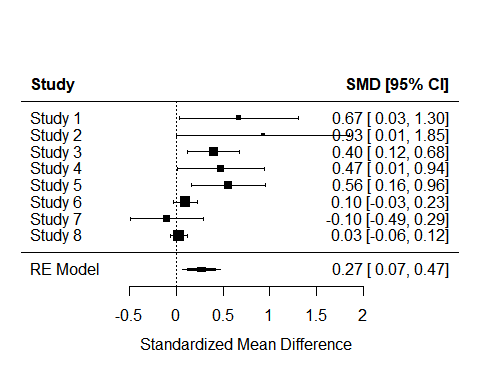
\includegraphics{2_general_structure_of_a_simulation__lesson_files/figure-latex/unnamed-chunk-11-1.pdf}

\hypertarget{a-better-way-using-dplyr-and-purrr}{%
\section{A better way using \{dplyr\} and
\{purrr\}}\label{a-better-way-using-dplyr-and-purrr}}

There are many other ways to implement simulations, using solutions
written in base R, purrr, and other packages such as SimDesign and
simhelpers.

My goal here is to teach you an approach that is both flexible and
intuitive for those who understand dplyr well already. It prioritizes
retaining all objects created within the simulation so that they are
visible and checkable, whereas other solutions make intermediate steps
invisible and abstract which is often difficult for new learners.

\begin{Shaded}
\begin{Highlighting}[]
\CommentTok{\# define experiment parameters}
\CommentTok{\# and use expand\_grid (the \{tidyr\} version of expand.grid) to create a data frame of all their permutations}
\CommentTok{\# note that each variable can have just one value or multiple values}
\NormalTok{experiment\_parameters\_grid }\OtherTok{\textless{}{-}} \FunctionTok{expand\_grid}\NormalTok{(}
  \AttributeTok{n\_control =} \FunctionTok{seq}\NormalTok{(}\AttributeTok{from =} \DecValTok{50}\NormalTok{, }\AttributeTok{to =} \DecValTok{250}\NormalTok{, }\AttributeTok{by =} \DecValTok{50}\NormalTok{),}
  \AttributeTok{n\_intervention =} \FunctionTok{seq}\NormalTok{(}\AttributeTok{from =} \DecValTok{50}\NormalTok{, }\AttributeTok{to =} \DecValTok{250}\NormalTok{, }\AttributeTok{by =} \DecValTok{50}\NormalTok{),}
  \AttributeTok{mean\_control =} \DecValTok{0}\NormalTok{,}
  \AttributeTok{mean\_intervention =} \FloatTok{0.5}\NormalTok{,}
  \AttributeTok{sd\_control =} \DecValTok{1}\NormalTok{,}
  \AttributeTok{sd\_intervention =} \DecValTok{1}\NormalTok{,}
  \AttributeTok{iteration =} \DecValTok{1}\SpecialCharTok{:}\DecValTok{100} \CommentTok{\# note this is a series not an integer, i.e., "1:100" not "100", as "100" would mean just one iteration called "100".}
\NormalTok{)}

  
\NormalTok{simulation }\OtherTok{\textless{}{-}} 
  \CommentTok{\# "using the experiment parameters..."}
\NormalTok{  experiment\_parameters\_grid }\SpecialCharTok{|\textgreater{}}
  
  \CommentTok{\# "...generate data using the data generating function and the parameters relevant to data generation ..."}
  \CommentTok{\# NB pmap() passes a list of parameters to the function listed as its second argument (generate\_data).}
  \CommentTok{\# when used inside a mutate call like this, its saying "for each row, create a new column (generated\_data)}
  \CommentTok{\# by calling a function (generate\_data) and use the following list of columns as its arguments.}
  \CommentTok{\# ensure the list orders the arguments in the same order as the function takes them, as they are passed to the function in this order!}
  \FunctionTok{mutate}\NormalTok{(}\AttributeTok{generated\_data =} \FunctionTok{pmap}\NormalTok{(}\FunctionTok{list}\NormalTok{(n\_control, }
\NormalTok{                                    n\_intervention,}
\NormalTok{                                    mean\_control,}
\NormalTok{                                    mean\_intervention,}
\NormalTok{                                    sd\_control,}
\NormalTok{                                    sd\_intervention),}
\NormalTok{                               generate\_data)) }\SpecialCharTok{|\textgreater{}}
  
  \CommentTok{\# "... then apply the analysis function to the generated data using the parameters relevant to analysis ..."}
  \CommentTok{\# again ensure they are listed in the correct order, as they are passed to the function in this order!}
  \FunctionTok{mutate}\NormalTok{(}\AttributeTok{analysis\_results =} \FunctionTok{pmap}\NormalTok{(}\FunctionTok{list}\NormalTok{(generated\_data),}
\NormalTok{                                 analyse\_data))}
  

\CommentTok{\# "... then summarise results across iterations"}
\NormalTok{simulation\_summary }\OtherTok{\textless{}{-}}\NormalTok{ simulation }\SpecialCharTok{|\textgreater{}}
  \CommentTok{\# convert this column in the df that is a nested data frame into columns in the df}
  \FunctionTok{unnest}\NormalTok{(analysis\_results) }\SpecialCharTok{|\textgreater{}} 
  \CommentTok{\# convert these variables into factors for plotting}
  \FunctionTok{mutate}\NormalTok{(}\AttributeTok{n\_control =} \FunctionTok{as.factor}\NormalTok{(n\_control), }
         \AttributeTok{n\_intervention =} \FunctionTok{as.factor}\NormalTok{(n\_intervention)) }\SpecialCharTok{|\textgreater{}}
  \CommentTok{\# for each level of n\_control and n\_intervention, calculate power (proportion of iterations where signficiant results were found)}
  \FunctionTok{group\_by}\NormalTok{(n\_control, }
\NormalTok{           n\_intervention) }\SpecialCharTok{|\textgreater{}}
  \FunctionTok{summarize}\NormalTok{(}\AttributeTok{power =} \FunctionTok{mean}\NormalTok{(p }\SpecialCharTok{\textless{}}\NormalTok{ .}\DecValTok{05}\NormalTok{), }\AttributeTok{.groups =} \StringTok{"drop"}\NormalTok{)}

\CommentTok{\# plot results}
\FunctionTok{ggplot}\NormalTok{(simulation\_summary, }\FunctionTok{aes}\NormalTok{(n\_control, power, }\AttributeTok{fill =}\NormalTok{ n\_intervention)) }\SpecialCharTok{+}
  \FunctionTok{geom\_col}\NormalTok{(}\AttributeTok{position =} \FunctionTok{position\_dodge}\NormalTok{(}\AttributeTok{width =} \FloatTok{0.4}\NormalTok{), }\AttributeTok{width =} \FloatTok{0.4}\NormalTok{) }\SpecialCharTok{+}
  \FunctionTok{scale\_fill\_viridis\_d}\NormalTok{(}\AttributeTok{option =} \StringTok{"mako"}\NormalTok{, }\AttributeTok{begin =} \FloatTok{0.3}\NormalTok{, }\AttributeTok{end =} \FloatTok{0.8}\NormalTok{, }
                       \AttributeTok{guide =} \FunctionTok{guide\_legend}\NormalTok{(}\AttributeTok{reverse =} \ConstantTok{TRUE}\NormalTok{)) }\SpecialCharTok{+}
  \FunctionTok{theme\_linedraw}\NormalTok{() }\SpecialCharTok{+}
  \FunctionTok{ggtitle}\NormalTok{(}\StringTok{"All conditions"}\NormalTok{) }\SpecialCharTok{+}
  \FunctionTok{ylab}\NormalTok{(}\StringTok{"Estimated statistical power"}\NormalTok{)}
\end{Highlighting}
\end{Shaded}

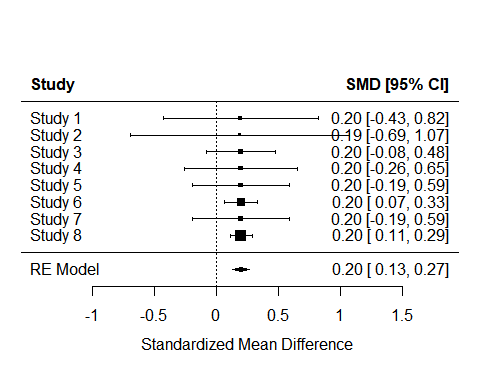
\includegraphics{2_general_structure_of_a_simulation__lesson_files/figure-latex/unnamed-chunk-12-1.pdf}

\begin{itemize}
\tightlist
\item
  Inspect the parameters grid to see how it contains a row for each
  iteration to be run, containing all the parameters for that iteration.
\item
  View the \texttt{simulation} data frame: notice that it saves the data
  and results from each iteration as a ``nested data frame'' column. You
  can click on each cell to open it and see the data frame contained.
\item
  It's really important to understand the pmap() call here. It allows us
  to effectively run the following code on each row, while avoiding
  using \texttt{rowwise()} because that can be much slower and cause
  issues later. However, it can help to see it implemented using
  rowwise() (without pmap()) to understand it. If it helps you to
  understand it, you can write your own simulations this way for the
  moment but note that they'll be slower to run.
\end{itemize}

\begin{Shaded}
\begin{Highlighting}[]
\NormalTok{simulation\_alt }\OtherTok{\textless{}{-}} 
  \CommentTok{\# "using the experiment parameters..."}
\NormalTok{  experiment\_parameters\_grid }\SpecialCharTok{|\textgreater{}}
  
  \CommentTok{\# "...generate data using the data generating function and the parameters relevant to data generation ..."}
  \FunctionTok{rowwise}\NormalTok{() }\SpecialCharTok{|\textgreater{}} \CommentTok{\# without pmap(), you need a rowwise() call to use only the values from this row as input in the next line.}
  \CommentTok{\# note how the output of generate\_data() has to be converted to a list() to be saved in a single cell.}
  \FunctionTok{mutate}\NormalTok{(}\AttributeTok{generated\_data =} \FunctionTok{list}\NormalTok{(}\FunctionTok{generate\_data}\NormalTok{(}\AttributeTok{n\_control =}\NormalTok{ n\_control, }
                                             \AttributeTok{n\_intervention =}\NormalTok{ n\_intervention,}
                                             \AttributeTok{mean\_control =}\NormalTok{ mean\_control,}
                                             \AttributeTok{mean\_intervention =}\NormalTok{ mean\_intervention,}
                                             \AttributeTok{sd\_control =}\NormalTok{ sd\_control,}
                                             \AttributeTok{sd\_intervention =}\NormalTok{ sd\_intervention))) }\SpecialCharTok{|\textgreater{}}
  
  \CommentTok{\# "... then apply the analysis function to the generated data using the parameters relevant to analysis ..."}
  \FunctionTok{mutate}\NormalTok{(}\AttributeTok{analysis\_results =} \FunctionTok{list}\NormalTok{(}\FunctionTok{analyse\_data}\NormalTok{(}\AttributeTok{data =}\NormalTok{ generated\_data))) }\SpecialCharTok{|\textgreater{}}
  \FunctionTok{ungroup}\NormalTok{() }\CommentTok{\# once the operations that need to be completed rowwise() are complete you should ungroup() the data again so it doesn\textquotesingle{}t have unintended consequences in later code.}
\end{Highlighting}
\end{Shaded}

\hypertarget{the-flexibility-of-this-approach}{%
\subsection{The flexibility of this
approach}\label{the-flexibility-of-this-approach}}

This approach where we (a) define a grid of all the parameters and
iterations we want to run, (b) map our data generation and analysis
functions onto each row, saving nested data frames each time, is
extremely scalable. By this, I mean that we can examine any other values
of these parameters that we like, or indeed change some parameters from
being static single parameters to having multiple ones (i.e.,
experimentally manipulate them), without having to write additional
for-loops to handle them.

For example, let's simulate more than one true effect size and see how
power changes with true effect size too.

\begin{Shaded}
\begin{Highlighting}[]
\CommentTok{\# define experiment parameters}
\NormalTok{experiment\_parameters\_grid }\OtherTok{\textless{}{-}} \FunctionTok{expand\_grid}\NormalTok{(}
  \AttributeTok{n\_control =} \FunctionTok{seq}\NormalTok{(}\AttributeTok{from =} \DecValTok{50}\NormalTok{, }\AttributeTok{to =} \DecValTok{250}\NormalTok{, }\AttributeTok{by =} \DecValTok{50}\NormalTok{),}
  \AttributeTok{n\_intervention =} \FunctionTok{seq}\NormalTok{(}\AttributeTok{from =} \DecValTok{50}\NormalTok{, }\AttributeTok{to =} \DecValTok{250}\NormalTok{, }\AttributeTok{by =} \DecValTok{50}\NormalTok{),}
  \AttributeTok{mean\_control =} \DecValTok{0}\NormalTok{,}
  \AttributeTok{mean\_intervention =} \FunctionTok{c}\NormalTok{(}\FloatTok{0.2}\NormalTok{, }\FloatTok{0.5}\NormalTok{, }\FloatTok{0.8}\NormalTok{), }\CommentTok{\# I\textquotesingle{}ve added additional values here for small, medium, \& large Cohen\textquotesingle{}s d  {-} this is the only change to the code}
  \AttributeTok{sd\_control =} \DecValTok{1}\NormalTok{,}
  \AttributeTok{sd\_intervention =} \DecValTok{1}\NormalTok{,}
  \AttributeTok{iteration =} \DecValTok{1}\SpecialCharTok{:}\DecValTok{100} 
\NormalTok{)}

\NormalTok{simulation }\OtherTok{\textless{}{-}} 
  \CommentTok{\# using the experiment parameters}
\NormalTok{  experiment\_parameters\_grid }\SpecialCharTok{|\textgreater{}}
  
  \CommentTok{\# generate data using the data generating function and the parameters relevant to data generation}
  \FunctionTok{mutate}\NormalTok{(}\AttributeTok{generated\_data =} \FunctionTok{pmap}\NormalTok{(}\FunctionTok{list}\NormalTok{(n\_control,}
\NormalTok{                                    n\_intervention,}
\NormalTok{                                    mean\_control,}
\NormalTok{                                    mean\_intervention,}
\NormalTok{                                    sd\_control,}
\NormalTok{                                    sd\_intervention),}
\NormalTok{                               generate\_data)) }\SpecialCharTok{|\textgreater{}}
  
  \CommentTok{\# apply the analysis function to the generated data using the parameters relevant to analysis}
  \FunctionTok{mutate}\NormalTok{(}\AttributeTok{analysis\_results =} \FunctionTok{pmap}\NormalTok{(}\FunctionTok{list}\NormalTok{(generated\_data),}
\NormalTok{                                 analyse\_data))}
  

\CommentTok{\# summarise results across iterations}
\NormalTok{simulation\_summary }\OtherTok{\textless{}{-}}\NormalTok{ simulation }\SpecialCharTok{|\textgreater{}}
  \FunctionTok{unnest}\NormalTok{(analysis\_results) }\SpecialCharTok{|\textgreater{}}
  \FunctionTok{mutate}\NormalTok{(}\AttributeTok{n\_control =} \FunctionTok{as.factor}\NormalTok{(n\_control),}
         \AttributeTok{n\_intervention =} \FunctionTok{as.factor}\NormalTok{(n\_intervention),}
         \AttributeTok{true\_effect =} \FunctionTok{paste}\NormalTok{(}\StringTok{"Cohen\textquotesingle{}s d ="}\NormalTok{, mean\_intervention)) }\SpecialCharTok{|\textgreater{}}
  \FunctionTok{group\_by}\NormalTok{(n\_control,}
\NormalTok{           n\_intervention,}
\NormalTok{           true\_effect) }\SpecialCharTok{|\textgreater{}}
  \FunctionTok{summarize}\NormalTok{(}\AttributeTok{power =} \FunctionTok{mean}\NormalTok{(p }\SpecialCharTok{\textless{}}\NormalTok{ .}\DecValTok{05}\NormalTok{), }\AttributeTok{.groups =} \StringTok{"drop"}\NormalTok{)}

\CommentTok{\# plot summary}
\FunctionTok{ggplot}\NormalTok{(simulation\_summary, }\FunctionTok{aes}\NormalTok{(n\_control, power, }\AttributeTok{fill =}\NormalTok{ n\_intervention)) }\SpecialCharTok{+}
  \FunctionTok{geom\_col}\NormalTok{(}\AttributeTok{position =} \FunctionTok{position\_dodge}\NormalTok{(}\AttributeTok{width =} \FloatTok{0.4}\NormalTok{), }\AttributeTok{width =} \FloatTok{0.4}\NormalTok{) }\SpecialCharTok{+}
  \FunctionTok{scale\_fill\_viridis\_d}\NormalTok{(}\AttributeTok{option =} \StringTok{"mako"}\NormalTok{, }\AttributeTok{begin =} \FloatTok{0.3}\NormalTok{, }\AttributeTok{end =} \FloatTok{0.8}\NormalTok{, }
                       \AttributeTok{guide =} \FunctionTok{guide\_legend}\NormalTok{(}\AttributeTok{reverse =} \ConstantTok{TRUE}\NormalTok{)) }\SpecialCharTok{+}
  \FunctionTok{theme\_linedraw}\NormalTok{() }\SpecialCharTok{+}
  \FunctionTok{ggtitle}\NormalTok{(}\StringTok{"All conditions"}\NormalTok{) }\SpecialCharTok{+}
  \FunctionTok{ylab}\NormalTok{(}\StringTok{"Estimated statistical power"}\NormalTok{) }\SpecialCharTok{+}
  \FunctionTok{facet\_wrap}\NormalTok{(}\SpecialCharTok{\textasciitilde{}}\NormalTok{ true\_effect)}
\end{Highlighting}
\end{Shaded}

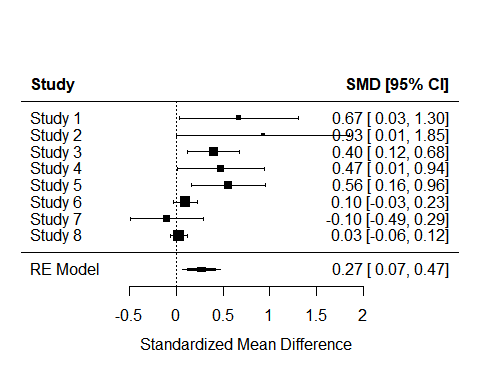
\includegraphics{2_general_structure_of_a_simulation__lesson_files/figure-latex/unnamed-chunk-14-1.pdf}

\hypertarget{extending-this-simulation}{%
\subsection{Extending this simulation}\label{extending-this-simulation}}

We saw above that this approach allows us to easily simulate additional
conditions simply by including them in our expand\_grid parameters. If
we want to simulate additional conditions or collect additional data
from, we can also easily modify our data generation or data analysis
functions to do this, (often) without having to change other components
of the simulation, or without having to change them much (e.g., by
adding additional parameters to the expand grid).

For example, if we want our analysis to save the p values but also the
Cohen's d effect sizes, we can modify the function to do this.

\begin{Shaded}
\begin{Highlighting}[]
\CommentTok{\# redefine the data generation function}
\NormalTok{generate\_data }\OtherTok{\textless{}{-}} \ControlFlowTok{function}\NormalTok{(n\_control, }\CommentTok{\# the parameters are now function arguments}
\NormalTok{                          n\_intervention,}
\NormalTok{                          mean\_control,}
\NormalTok{                          mean\_intervention,}
\NormalTok{                          sd\_control,}
\NormalTok{                          sd\_intervention) \{}
  
\NormalTok{  data }\OtherTok{\textless{}{-}} 
    \FunctionTok{bind\_rows}\NormalTok{(}
      \FunctionTok{tibble}\NormalTok{(}\AttributeTok{condition =} \StringTok{"control"}\NormalTok{,}
             \AttributeTok{score =} \FunctionTok{rnorm}\NormalTok{(}\AttributeTok{n =}\NormalTok{ n\_control, }\AttributeTok{mean =}\NormalTok{ mean\_control, }\AttributeTok{sd =}\NormalTok{ sd\_control)),}
      \FunctionTok{tibble}\NormalTok{(}\AttributeTok{condition =} \StringTok{"intervention"}\NormalTok{,}
             \AttributeTok{score =} \FunctionTok{rnorm}\NormalTok{(}\AttributeTok{n =}\NormalTok{ n\_intervention, }\AttributeTok{mean =}\NormalTok{ mean\_intervention, }\AttributeTok{sd =}\NormalTok{ sd\_intervention))}
\NormalTok{    ) }\SpecialCharTok{|\textgreater{}}
  \CommentTok{\# new addition: control\textquotesingle{}s factor levels must be ordered so that intervention is the first level and control is the second}
  \CommentTok{\# this ensures that positive cohen\textquotesingle{}s d values refer to intervention \textgreater{} control and not the other way around.}
  \FunctionTok{mutate}\NormalTok{(}\AttributeTok{condition =} \FunctionTok{fct\_relevel}\NormalTok{(condition, }\StringTok{"intervention"}\NormalTok{, }\StringTok{"control"}\NormalTok{))}
  
  \FunctionTok{return}\NormalTok{(data)}
\NormalTok{\}}

\CommentTok{\# redefine the analysis function}
\NormalTok{analyse\_data }\OtherTok{\textless{}{-}} \ControlFlowTok{function}\NormalTok{(data) \{}
  \CommentTok{\# dependencies}
  \FunctionTok{require}\NormalTok{(effsize)}
  
\NormalTok{  res\_t\_test }\OtherTok{\textless{}{-}} \FunctionTok{t.test}\NormalTok{(}\AttributeTok{formula =}\NormalTok{ score }\SpecialCharTok{\textasciitilde{}}\NormalTok{ condition, }
                       \AttributeTok{data =}\NormalTok{ data,}
                       \AttributeTok{var.equal =} \ConstantTok{TRUE}\NormalTok{,}
                       \AttributeTok{alternative =} \StringTok{"two.sided"}\NormalTok{)}
  
\NormalTok{  res\_cohens\_d }\OtherTok{\textless{}{-}}\NormalTok{ effsize}\SpecialCharTok{::}\FunctionTok{cohen.d}\NormalTok{(}\AttributeTok{formula =}\NormalTok{ score }\SpecialCharTok{\textasciitilde{}}\NormalTok{ condition,  }\CommentTok{\# new addition: also fit cohen\textquotesingle{}s d}
                                   \AttributeTok{within =} \ConstantTok{FALSE}\NormalTok{,}
                                   \AttributeTok{data =}\NormalTok{ data)}
  
\NormalTok{  res }\OtherTok{\textless{}{-}} \FunctionTok{tibble}\NormalTok{(}\AttributeTok{p =}\NormalTok{ res\_t\_test}\SpecialCharTok{$}\NormalTok{p.value, }
                \AttributeTok{cohens\_d =}\NormalTok{ res\_cohens\_d}\SpecialCharTok{$}\NormalTok{estimate,  }\CommentTok{\# new addition: save cohen\textquotesingle{}s d and its 95\% CIs to the results tibble}
                \AttributeTok{cohens\_d\_ci\_lower =}\NormalTok{ res\_cohens\_d}\SpecialCharTok{$}\NormalTok{conf.int[}\StringTok{"lower"}\NormalTok{],}
                \AttributeTok{cohens\_d\_ci\_upper =}\NormalTok{ res\_cohens\_d}\SpecialCharTok{$}\NormalTok{conf.int[}\StringTok{"upper"}\NormalTok{])}
  
  \FunctionTok{return}\NormalTok{(res)}
\NormalTok{\}}


\CommentTok{\# the code for running the simulation remains unchanged:}

\CommentTok{\# define experiment parameters}
\NormalTok{experiment\_parameters\_grid }\OtherTok{\textless{}{-}} \FunctionTok{expand\_grid}\NormalTok{(}
  \AttributeTok{n\_control =} \FunctionTok{seq}\NormalTok{(}\AttributeTok{from =} \DecValTok{50}\NormalTok{, }\AttributeTok{to =} \DecValTok{250}\NormalTok{, }\AttributeTok{by =} \DecValTok{50}\NormalTok{),}
  \AttributeTok{n\_intervention =} \FunctionTok{seq}\NormalTok{(}\AttributeTok{from =} \DecValTok{50}\NormalTok{, }\AttributeTok{to =} \DecValTok{250}\NormalTok{, }\AttributeTok{by =} \DecValTok{50}\NormalTok{),}
  \AttributeTok{mean\_control =} \DecValTok{0}\NormalTok{,}
  \AttributeTok{mean\_intervention =} \FunctionTok{c}\NormalTok{(}\FloatTok{0.2}\NormalTok{, }\FloatTok{0.5}\NormalTok{, }\FloatTok{0.8}\NormalTok{), }\CommentTok{\# small, medium, large Cohen\textquotesingle{}s d }
  \AttributeTok{sd\_control =} \DecValTok{1}\NormalTok{,}
  \AttributeTok{sd\_intervention =} \DecValTok{1}\NormalTok{,}
  \AttributeTok{iteration =} \DecValTok{1}\SpecialCharTok{:}\DecValTok{100} 
\NormalTok{)}

\CommentTok{\# run simulation}
\NormalTok{simulation }\OtherTok{\textless{}{-}} 
  \CommentTok{\# using the experiment parameters}
\NormalTok{  experiment\_parameters\_grid }\SpecialCharTok{|\textgreater{}}
  
  \CommentTok{\# generate data using the data generating function and the parameters relevant to data generation}
  \FunctionTok{mutate}\NormalTok{(}\AttributeTok{generated\_data =} \FunctionTok{pmap}\NormalTok{(}\FunctionTok{list}\NormalTok{(n\_control,}
\NormalTok{                                    n\_intervention,}
\NormalTok{                                    mean\_control,}
\NormalTok{                                    mean\_intervention,}
\NormalTok{                                    sd\_control,}
\NormalTok{                                    sd\_intervention),}
\NormalTok{                               generate\_data)) }\SpecialCharTok{|\textgreater{}}
  
  \CommentTok{\# apply the analysis function to the generated data using the parameters relevant to analysis}
  \FunctionTok{mutate}\NormalTok{(}\AttributeTok{analysis\_results =} \FunctionTok{pmap}\NormalTok{(}\FunctionTok{list}\NormalTok{(generated\_data),}
\NormalTok{                                 analyse\_data))}
  

\CommentTok{\# summarise across iterations }
\NormalTok{simulation\_summary }\OtherTok{\textless{}{-}}\NormalTok{ simulation }\SpecialCharTok{|\textgreater{}}
  \FunctionTok{unnest}\NormalTok{(analysis\_results) }\SpecialCharTok{|\textgreater{}}
  \FunctionTok{mutate}\NormalTok{(}\AttributeTok{n\_control =} \FunctionTok{as.factor}\NormalTok{(n\_control),}
         \AttributeTok{n\_intervention =} \FunctionTok{as.factor}\NormalTok{(n\_intervention),}
         \AttributeTok{true\_effect =} \FunctionTok{paste}\NormalTok{(}\StringTok{"Cohen\textquotesingle{}s d ="}\NormalTok{, mean\_intervention)) }\SpecialCharTok{|\textgreater{}}
  \FunctionTok{group\_by}\NormalTok{(n\_control,}
\NormalTok{           n\_intervention,}
\NormalTok{           true\_effect) }\SpecialCharTok{|\textgreater{}}
  \FunctionTok{summarize}\NormalTok{(}\AttributeTok{power =} \FunctionTok{mean}\NormalTok{(p }\SpecialCharTok{\textless{}}\NormalTok{ .}\DecValTok{05}\NormalTok{), }\CommentTok{\# power: proportion of iterations where significant results were found when true effect is != zero.}
            \CommentTok{\# new: mean half{-}CI{-}width. ie with this sample size, how wide are its 95\% CIs, ± the point estimate?}
            \AttributeTok{mean\_cohens\_d\_precision =} \FunctionTok{mean}\NormalTok{((cohens\_d\_ci\_upper }\SpecialCharTok{{-}}\NormalTok{ cohens\_d\_ci\_lower)}\SpecialCharTok{/}\DecValTok{2}\NormalTok{), }
            \AttributeTok{.groups =} \StringTok{"drop"}\NormalTok{)}

\CommentTok{\# plot power }
\FunctionTok{ggplot}\NormalTok{(simulation\_summary, }\FunctionTok{aes}\NormalTok{(n\_control, power, }\AttributeTok{fill =}\NormalTok{ n\_intervention)) }\SpecialCharTok{+}
  \FunctionTok{geom\_col}\NormalTok{(}\AttributeTok{position =} \FunctionTok{position\_dodge}\NormalTok{(}\AttributeTok{width =} \FloatTok{0.4}\NormalTok{), }\AttributeTok{width =} \FloatTok{0.4}\NormalTok{) }\SpecialCharTok{+}
  \FunctionTok{scale\_fill\_viridis\_d}\NormalTok{(}\AttributeTok{option =} \StringTok{"mako"}\NormalTok{, }\AttributeTok{begin =} \FloatTok{0.3}\NormalTok{, }\AttributeTok{end =} \FloatTok{0.8}\NormalTok{, }
                       \AttributeTok{guide =} \FunctionTok{guide\_legend}\NormalTok{(}\AttributeTok{reverse =} \ConstantTok{TRUE}\NormalTok{)) }\SpecialCharTok{+}
  \FunctionTok{theme\_linedraw}\NormalTok{() }\SpecialCharTok{+}
  \FunctionTok{ggtitle}\NormalTok{(}\StringTok{"All conditions"}\NormalTok{) }\SpecialCharTok{+}
  \FunctionTok{ylab}\NormalTok{(}\StringTok{"Estimated statistical power"}\NormalTok{) }\SpecialCharTok{+}
  \FunctionTok{facet\_wrap}\NormalTok{(}\SpecialCharTok{\textasciitilde{}}\NormalTok{ true\_effect)}
\end{Highlighting}
\end{Shaded}

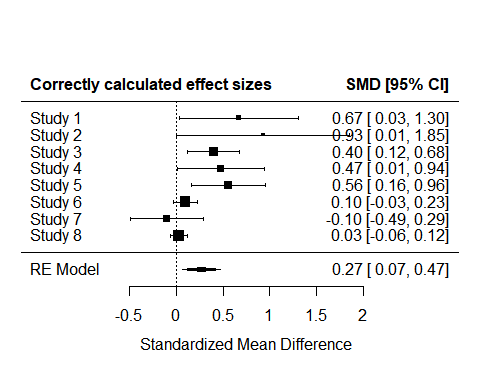
\includegraphics{2_general_structure_of_a_simulation__lesson_files/figure-latex/unnamed-chunk-15-1.pdf}

\begin{Shaded}
\begin{Highlighting}[]
\CommentTok{\# new plot: precision of cohen\textquotesingle{}s d}
\FunctionTok{ggplot}\NormalTok{(simulation\_summary, }\FunctionTok{aes}\NormalTok{(n\_control, mean\_cohens\_d\_precision, }\AttributeTok{fill =}\NormalTok{ n\_intervention)) }\SpecialCharTok{+}
  \FunctionTok{geom\_col}\NormalTok{(}\AttributeTok{position =} \FunctionTok{position\_dodge}\NormalTok{(}\AttributeTok{width =} \FloatTok{0.4}\NormalTok{), }\AttributeTok{width =} \FloatTok{0.4}\NormalTok{) }\SpecialCharTok{+}
  \FunctionTok{scale\_fill\_viridis\_d}\NormalTok{(}\AttributeTok{option =} \StringTok{"mako"}\NormalTok{, }\AttributeTok{begin =} \FloatTok{0.3}\NormalTok{, }\AttributeTok{end =} \FloatTok{0.8}\NormalTok{, }
                       \AttributeTok{guide =} \FunctionTok{guide\_legend}\NormalTok{(}\AttributeTok{reverse =} \ConstantTok{TRUE}\NormalTok{)) }\SpecialCharTok{+}
  \FunctionTok{theme\_linedraw}\NormalTok{() }\SpecialCharTok{+}
  \FunctionTok{ggtitle}\NormalTok{(}\StringTok{"All conditions"}\NormalTok{) }\SpecialCharTok{+}
  \FunctionTok{ylab}\NormalTok{(}\StringTok{"Precision of Cohen\textquotesingle{}s d}\SpecialCharTok{\textbackslash{}n}\StringTok{(mean half{-}95\% CI width)"}\NormalTok{) }\SpecialCharTok{+}
  \FunctionTok{facet\_wrap}\NormalTok{(}\SpecialCharTok{\textasciitilde{}}\NormalTok{ true\_effect)}
\end{Highlighting}
\end{Shaded}

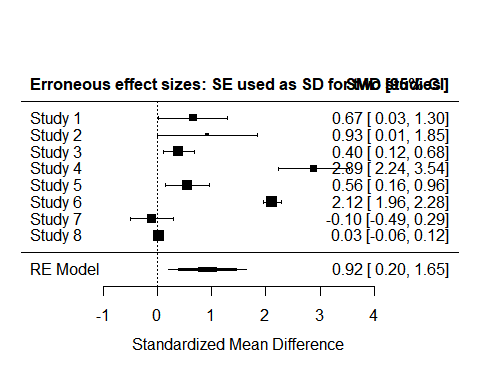
\includegraphics{2_general_structure_of_a_simulation__lesson_files/figure-latex/unnamed-chunk-15-2.pdf}

\hypertarget{putting-it-all-together}{%
\section{Putting it all together}\label{putting-it-all-together}}

Now let's bring all the code together and run the simulation for real.
We'll improve two things while we do it.

\emph{Issue 1}

You might have noticed that sometimes the results of the simulations
above have strange results between the sample-size conditions. E.g.,
some conditions with higher sample sizes have slighlty lower estimated
power. This shouldn't be the case, as high sample sizes = more power.
Why might this be the case?

Because, just like in an experiment with human participants, your sample
size matters. We have only collected data from 100 iterations, and so
the standard errors around each estimate will still be quite large. In
the final simulation below, we'll set \texttt{iterations} to
\texttt{1000} so that we have a lot more (simulated) data to base our
inferences on. Note that this may take a minute or two to run depending
on how fast your computer is. In general, simulations can be
computationally intensive to run as you're applying an analysis not once
but thousands of times.

\emph{Issue 2}

When you build simulations iteratively like we did above, its easy to
lose track of which code is actually necessary to the final simulation
vs.~which bits were part of your own learning process. If you don't
clean up your workflow every now and again, you will end up with
\href{https://en.wikipedia.org/wiki/Spaghetti_code}{spaghetti code} that
other people can't use, understand, or debug - and `other people' often
includes you yourself a few months from now.

So, in the below chunk, I pull together all the necessary code into (and
no unnecessary code), and use \texttt{rm(list\ =\ ls())} to remove all
previously saved objects from our R environment to ensure that we aren't
carrying over old versions of functions. This ensures that the contents
of this chunk alone represent a working simulation.

\begin{Shaded}
\begin{Highlighting}[]
\CommentTok{\# remove all objects from environment {-}{-}{-}{-}}
\FunctionTok{rm}\NormalTok{(}\AttributeTok{list =} \FunctionTok{ls}\NormalTok{())}


\CommentTok{\# dependencies {-}{-}{-}{-}}
\CommentTok{\# repeated here for the sake of completeness }

\FunctionTok{library}\NormalTok{(tidyr)}
\FunctionTok{library}\NormalTok{(dplyr)}
\FunctionTok{library}\NormalTok{(forcats)}
\FunctionTok{library}\NormalTok{(readr)}
\FunctionTok{library}\NormalTok{(purrr) }
\FunctionTok{library}\NormalTok{(ggplot2)}
\FunctionTok{library}\NormalTok{(effsize)}


\CommentTok{\# set the seed {-}{-}{-}{-}}
\CommentTok{\# for the pseudo random number generator to make results reproducible}
\FunctionTok{set.seed}\NormalTok{(}\DecValTok{42}\NormalTok{)}


\CommentTok{\# define data generating function {-}{-}{-}{-}}
\NormalTok{generate\_data }\OtherTok{\textless{}{-}} \ControlFlowTok{function}\NormalTok{(n\_control,}
\NormalTok{                          n\_intervention,}
\NormalTok{                          mean\_control,}
\NormalTok{                          mean\_intervention,}
\NormalTok{                          sd\_control,}
\NormalTok{                          sd\_intervention) \{}
  
\NormalTok{  data }\OtherTok{\textless{}{-}} 
    \FunctionTok{bind\_rows}\NormalTok{(}
      \FunctionTok{tibble}\NormalTok{(}\AttributeTok{condition =} \StringTok{"control"}\NormalTok{,}
             \AttributeTok{score =} \FunctionTok{rnorm}\NormalTok{(}\AttributeTok{n =}\NormalTok{ n\_control, }\AttributeTok{mean =}\NormalTok{ mean\_control, }\AttributeTok{sd =}\NormalTok{ sd\_control)),}
      \FunctionTok{tibble}\NormalTok{(}\AttributeTok{condition =} \StringTok{"intervention"}\NormalTok{,}
             \AttributeTok{score =} \FunctionTok{rnorm}\NormalTok{(}\AttributeTok{n =}\NormalTok{ n\_intervention, }\AttributeTok{mean =}\NormalTok{ mean\_intervention, }\AttributeTok{sd =}\NormalTok{ sd\_intervention))}
\NormalTok{    ) }\SpecialCharTok{|\textgreater{}}
    \CommentTok{\# control\textquotesingle{}s factor levels must be ordered so that intervention is the first level and control is the second}
    \CommentTok{\# this ensures that positive cohen\textquotesingle{}s d values refer to intervention \textgreater{} control and not the other way around.}
    \FunctionTok{mutate}\NormalTok{(}\AttributeTok{condition =} \FunctionTok{fct\_relevel}\NormalTok{(condition, }\StringTok{"intervention"}\NormalTok{, }\StringTok{"control"}\NormalTok{))}
  
  \FunctionTok{return}\NormalTok{(data)}
\NormalTok{\}}


\CommentTok{\# define data analysis function {-}{-}{-}{-}}
\NormalTok{analyse\_data }\OtherTok{\textless{}{-}} \ControlFlowTok{function}\NormalTok{(data) \{}
  \CommentTok{\# dependencies}
  \FunctionTok{require}\NormalTok{(effsize)}
  
\NormalTok{  res\_t\_test }\OtherTok{\textless{}{-}} \FunctionTok{t.test}\NormalTok{(}\AttributeTok{formula =}\NormalTok{ score }\SpecialCharTok{\textasciitilde{}}\NormalTok{ condition, }
                       \AttributeTok{data =}\NormalTok{ data,}
                       \AttributeTok{var.equal =} \ConstantTok{TRUE}\NormalTok{,}
                       \AttributeTok{alternative =} \StringTok{"two.sided"}\NormalTok{)}
  
\NormalTok{  res\_cohens\_d }\OtherTok{\textless{}{-}}\NormalTok{ effsize}\SpecialCharTok{::}\FunctionTok{cohen.d}\NormalTok{(}\AttributeTok{formula =}\NormalTok{ score }\SpecialCharTok{\textasciitilde{}}\NormalTok{ condition,  }\CommentTok{\# new addition: also fit cohen\textquotesingle{}s d}
                                   \AttributeTok{within =} \ConstantTok{FALSE}\NormalTok{,}
                                   \AttributeTok{data =}\NormalTok{ data)}
  
\NormalTok{  res }\OtherTok{\textless{}{-}} \FunctionTok{tibble}\NormalTok{(}\AttributeTok{p =}\NormalTok{ res\_t\_test}\SpecialCharTok{$}\NormalTok{p.value, }
                \AttributeTok{cohens\_d =}\NormalTok{ res\_cohens\_d}\SpecialCharTok{$}\NormalTok{estimate,  }\CommentTok{\# new addition: save cohen\textquotesingle{}s d and its 95\% CIs to the results tibble}
                \AttributeTok{cohens\_d\_ci\_lower =}\NormalTok{ res\_cohens\_d}\SpecialCharTok{$}\NormalTok{conf.int[}\StringTok{"lower"}\NormalTok{],}
                \AttributeTok{cohens\_d\_ci\_upper =}\NormalTok{ res\_cohens\_d}\SpecialCharTok{$}\NormalTok{conf.int[}\StringTok{"upper"}\NormalTok{])}
  
  \FunctionTok{return}\NormalTok{(res)}
\NormalTok{\}}


\CommentTok{\# define experiment parameters {-}{-}{-}{-}}
\NormalTok{experiment\_parameters\_grid }\OtherTok{\textless{}{-}} \FunctionTok{expand\_grid}\NormalTok{(}
  \AttributeTok{n\_control =} \FunctionTok{seq}\NormalTok{(}\AttributeTok{from =} \DecValTok{50}\NormalTok{, }\AttributeTok{to =} \DecValTok{250}\NormalTok{, }\AttributeTok{by =} \DecValTok{50}\NormalTok{),}
  \AttributeTok{n\_intervention =} \FunctionTok{seq}\NormalTok{(}\AttributeTok{from =} \DecValTok{50}\NormalTok{, }\AttributeTok{to =} \DecValTok{250}\NormalTok{, }\AttributeTok{by =} \DecValTok{50}\NormalTok{),}
  \AttributeTok{mean\_control =} \DecValTok{0}\NormalTok{,}
  \AttributeTok{mean\_intervention =} \FunctionTok{c}\NormalTok{(}\FloatTok{0.2}\NormalTok{, }\FloatTok{0.5}\NormalTok{, }\FloatTok{0.8}\NormalTok{), }\CommentTok{\# small, medium, large Cohen\textquotesingle{}s d}
  \AttributeTok{sd\_control =} \DecValTok{1}\NormalTok{,}
  \AttributeTok{sd\_intervention =} \DecValTok{1}\NormalTok{,}
  \AttributeTok{iteration =} \DecValTok{1}\SpecialCharTok{:}\DecValTok{1000} \CommentTok{\# increased number of iterations for more stable estimates. NB real stimulation are often much higher again.}
\NormalTok{)}


\CommentTok{\# run simulation {-}{-}{-}{-}}
\NormalTok{simulation }\OtherTok{\textless{}{-}} 
  \CommentTok{\# using the experiment parameters}
\NormalTok{  experiment\_parameters\_grid }\SpecialCharTok{|\textgreater{}}
  
  \CommentTok{\# generate data using the data generating function and the parameters relevant to data generation}
  \FunctionTok{mutate}\NormalTok{(}\AttributeTok{generated\_data =} \FunctionTok{pmap}\NormalTok{(}\FunctionTok{list}\NormalTok{(n\_control,}
\NormalTok{                                    n\_intervention,}
\NormalTok{                                    mean\_control,}
\NormalTok{                                    mean\_intervention,}
\NormalTok{                                    sd\_control,}
\NormalTok{                                    sd\_intervention),}
\NormalTok{                               generate\_data)) }\SpecialCharTok{|\textgreater{}}
  
  \CommentTok{\# apply the analysis function to the generated data using the parameters relevant to analysis}
  \FunctionTok{mutate}\NormalTok{(}\AttributeTok{analysis\_results =} \FunctionTok{pmap}\NormalTok{(}\FunctionTok{list}\NormalTok{(generated\_data),}
\NormalTok{                                 analyse\_data))}
  

\CommentTok{\# \# optional: save results to disk}
\CommentTok{\# write\_rds(simulation, "simulation\_1\_results.rds")}
\CommentTok{\# \# read from disk in future if it exists already}
\CommentTok{\# simulation \textless{}{-} read\_rds("simulation\_1\_results.rds")}


\CommentTok{\# summarise simulation results over the iterations {-}{-}{-}{-}}
\DocumentationTok{\#\# estimate power  }
\DocumentationTok{\#\# ie what proportion of p values are significant (\textless{} .05)}
\NormalTok{simulation\_summary }\OtherTok{\textless{}{-}}\NormalTok{ simulation }\SpecialCharTok{|\textgreater{}}
  \FunctionTok{unnest}\NormalTok{(analysis\_results) }\SpecialCharTok{|\textgreater{}}
  \FunctionTok{mutate}\NormalTok{(}\AttributeTok{n\_control =} \FunctionTok{as.factor}\NormalTok{(n\_control),}
         \AttributeTok{n\_intervention =} \FunctionTok{as.factor}\NormalTok{(n\_intervention),}
         \AttributeTok{true\_effect =} \FunctionTok{paste}\NormalTok{(}\StringTok{"Cohen\textquotesingle{}s d ="}\NormalTok{, mean\_intervention)) }\SpecialCharTok{|\textgreater{}}
  \FunctionTok{group\_by}\NormalTok{(n\_control,}
\NormalTok{           n\_intervention,}
\NormalTok{           true\_effect) }\SpecialCharTok{|\textgreater{}}
  \FunctionTok{summarize}\NormalTok{(}\AttributeTok{power =} \FunctionTok{mean}\NormalTok{(p }\SpecialCharTok{\textless{}}\NormalTok{ .}\DecValTok{05}\NormalTok{), }
            \AttributeTok{mean\_cohens\_d\_precision =} \FunctionTok{mean}\NormalTok{((cohens\_d\_ci\_upper }\SpecialCharTok{{-}}\NormalTok{ cohens\_d\_ci\_lower)}\SpecialCharTok{/}\DecValTok{2}\NormalTok{),}
            \AttributeTok{.groups =} \StringTok{"drop"}\NormalTok{)}

\CommentTok{\# plot power}
\FunctionTok{ggplot}\NormalTok{(simulation\_summary, }\FunctionTok{aes}\NormalTok{(n\_control, power, }\AttributeTok{fill =}\NormalTok{ n\_intervention)) }\SpecialCharTok{+}
  \FunctionTok{geom\_col}\NormalTok{(}\AttributeTok{position =} \FunctionTok{position\_dodge}\NormalTok{(}\AttributeTok{width =} \FloatTok{0.4}\NormalTok{), }\AttributeTok{width =} \FloatTok{0.4}\NormalTok{) }\SpecialCharTok{+}
  \FunctionTok{scale\_fill\_viridis\_d}\NormalTok{(}\AttributeTok{option =} \StringTok{"mako"}\NormalTok{, }\AttributeTok{begin =} \FloatTok{0.3}\NormalTok{, }\AttributeTok{end =} \FloatTok{0.8}\NormalTok{, }
                       \AttributeTok{guide =} \FunctionTok{guide\_legend}\NormalTok{(}\AttributeTok{reverse =} \ConstantTok{TRUE}\NormalTok{)) }\SpecialCharTok{+}
  \FunctionTok{theme\_linedraw}\NormalTok{() }\SpecialCharTok{+}
  \FunctionTok{ggtitle}\NormalTok{(}\StringTok{"All conditions"}\NormalTok{) }\SpecialCharTok{+}
  \FunctionTok{ylab}\NormalTok{(}\StringTok{"Estimated statistical power"}\NormalTok{) }\SpecialCharTok{+}
  \FunctionTok{facet\_wrap}\NormalTok{(}\SpecialCharTok{\textasciitilde{}}\NormalTok{ true\_effect)}
\end{Highlighting}
\end{Shaded}

\includegraphics{2_general_structure_of_a_simulation__lesson_files/figure-latex/unnamed-chunk-16-1.pdf}

\begin{Shaded}
\begin{Highlighting}[]
\CommentTok{\# plot precision}
\FunctionTok{ggplot}\NormalTok{(simulation\_summary, }\FunctionTok{aes}\NormalTok{(n\_control, mean\_cohens\_d\_precision, }\AttributeTok{fill =}\NormalTok{ n\_intervention)) }\SpecialCharTok{+}
  \FunctionTok{geom\_col}\NormalTok{(}\AttributeTok{position =} \FunctionTok{position\_dodge}\NormalTok{(}\AttributeTok{width =} \FloatTok{0.4}\NormalTok{), }\AttributeTok{width =} \FloatTok{0.4}\NormalTok{) }\SpecialCharTok{+}
  \FunctionTok{scale\_fill\_viridis\_d}\NormalTok{(}\AttributeTok{option =} \StringTok{"mako"}\NormalTok{, }\AttributeTok{begin =} \FloatTok{0.3}\NormalTok{, }\AttributeTok{end =} \FloatTok{0.8}\NormalTok{, }
                       \AttributeTok{guide =} \FunctionTok{guide\_legend}\NormalTok{(}\AttributeTok{reverse =} \ConstantTok{TRUE}\NormalTok{)) }\SpecialCharTok{+}
  \FunctionTok{theme\_linedraw}\NormalTok{() }\SpecialCharTok{+}
  \FunctionTok{ggtitle}\NormalTok{(}\StringTok{"All conditions"}\NormalTok{) }\SpecialCharTok{+}
  \FunctionTok{ylab}\NormalTok{(}\StringTok{"Precision of Cohen\textquotesingle{}s d}\SpecialCharTok{\textbackslash{}n}\StringTok{(mean half{-}95\% CI width)"}\NormalTok{) }\SpecialCharTok{+}
  \FunctionTok{facet\_wrap}\NormalTok{(}\SpecialCharTok{\textasciitilde{}}\NormalTok{ true\_effect)}
\end{Highlighting}
\end{Shaded}

\includegraphics{2_general_structure_of_a_simulation__lesson_files/figure-latex/unnamed-chunk-16-2.pdf}

\hypertarget{make-inferences-across-experimental-conditions}{%
\section{Make inferences across experimental
conditions}\label{make-inferences-across-experimental-conditions}}

Now that we've learned something about how to build simulations
generally, what can we learn from this stimulation specifically?

Let's plot only those simulations where the total sample size between
the two conditions is n = 300. By doing this, we are effectively
simulating the impact of (un)balanced sample sizes on an independent
t-test's statistical power. That is, all the columns refer to the same
total sample size, but they differ in the number allotted to the control
vs intervention conditions.

\begin{Shaded}
\begin{Highlighting}[]
\NormalTok{simulation }\SpecialCharTok{|\textgreater{}}
  \FunctionTok{unnest}\NormalTok{(analysis\_results) }\SpecialCharTok{|\textgreater{}}
  \FunctionTok{filter}\NormalTok{(n\_control }\SpecialCharTok{+}\NormalTok{ n\_intervention }\SpecialCharTok{==} \DecValTok{300}\NormalTok{) }\SpecialCharTok{|\textgreater{}} \CommentTok{\# subset only the conditions where total n = 300}
  \FunctionTok{mutate}\NormalTok{(}\AttributeTok{n\_control =} \FunctionTok{as.factor}\NormalTok{(n\_control),}
         \AttributeTok{n\_intervention =} \FunctionTok{as.factor}\NormalTok{(n\_intervention),}
         \AttributeTok{true\_effect =} \FunctionTok{paste}\NormalTok{(}\StringTok{"Cohen\textquotesingle{}s d ="}\NormalTok{, mean\_intervention)) }\SpecialCharTok{|\textgreater{}}
  \FunctionTok{group\_by}\NormalTok{(n\_control,}
\NormalTok{           n\_intervention,}
\NormalTok{           true\_effect) }\SpecialCharTok{|\textgreater{}}
  \FunctionTok{summarize}\NormalTok{(}\AttributeTok{power =} \FunctionTok{mean}\NormalTok{(p }\SpecialCharTok{\textless{}}\NormalTok{ .}\DecValTok{05}\NormalTok{), }\AttributeTok{.groups =} \StringTok{"drop"}\NormalTok{) }\SpecialCharTok{|\textgreater{}}
  \FunctionTok{ggplot}\NormalTok{(}\FunctionTok{aes}\NormalTok{(n\_control, power, }\AttributeTok{fill =}\NormalTok{ n\_intervention)) }\SpecialCharTok{+}
  \FunctionTok{geom\_col}\NormalTok{(}\AttributeTok{position =} \FunctionTok{position\_dodge}\NormalTok{(}\AttributeTok{width =} \FloatTok{0.4}\NormalTok{), }\AttributeTok{width =} \FloatTok{0.4}\NormalTok{) }\SpecialCharTok{+}
  \FunctionTok{scale\_fill\_viridis\_d}\NormalTok{(}\AttributeTok{option =} \StringTok{"mako"}\NormalTok{, }\AttributeTok{begin =} \FloatTok{0.3}\NormalTok{, }\AttributeTok{end =} \FloatTok{0.8}\NormalTok{, }\AttributeTok{direction =} \SpecialCharTok{{-}}\DecValTok{1}\NormalTok{,}
                       \AttributeTok{guide =} \FunctionTok{guide\_legend}\NormalTok{(}\AttributeTok{reverse =} \ConstantTok{TRUE}\NormalTok{)) }\SpecialCharTok{+}
  \FunctionTok{theme\_linedraw}\NormalTok{() }\SpecialCharTok{+}
  \FunctionTok{ggtitle}\NormalTok{(}\StringTok{"Conditions where total N = 300"}\NormalTok{) }\SpecialCharTok{+}
  \FunctionTok{ylab}\NormalTok{(}\StringTok{"Estimated statistical power"}\NormalTok{) }\SpecialCharTok{+}
  \FunctionTok{facet\_wrap}\NormalTok{(}\SpecialCharTok{\textasciitilde{}}\NormalTok{ true\_effect)}
\end{Highlighting}
\end{Shaded}

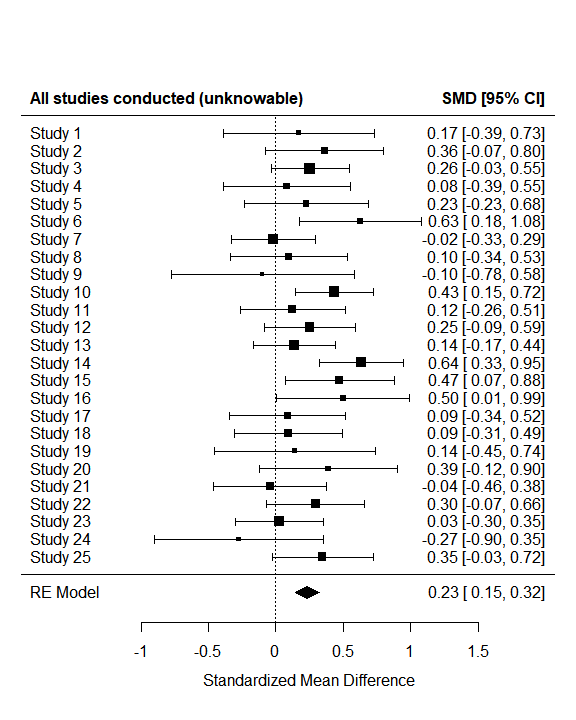
\includegraphics{2_general_structure_of_a_simulation__lesson_files/figure-latex/unnamed-chunk-17-1.pdf}

This shows that power is highest when the two conditions have balanced
sample sizes, and tells us something about how much power decreases when
sample sizes are unbalanced.

Note however that larger sample sizes are always preferable over smaller
ones! I have seen students make this mistake recently. Don't ever not
have a larger sample size if you can. E.g., compare power in the above
conditions where total n = 300 with the below conditions where total n =
150, you gain more power from additional unbalanced participants than
you lost due to imbalance.

\begin{Shaded}
\begin{Highlighting}[]
\NormalTok{simulation }\SpecialCharTok{|\textgreater{}}
  \FunctionTok{unnest}\NormalTok{(analysis\_results) }\SpecialCharTok{|\textgreater{}}
  \FunctionTok{filter}\NormalTok{(n\_control }\SpecialCharTok{+}\NormalTok{ n\_intervention }\SpecialCharTok{==} \DecValTok{150}\NormalTok{) }\SpecialCharTok{|\textgreater{}} \CommentTok{\# subset only the conditions where total n = 150}
  \FunctionTok{mutate}\NormalTok{(}\AttributeTok{n\_control =} \FunctionTok{as.factor}\NormalTok{(n\_control),}
         \AttributeTok{n\_intervention =} \FunctionTok{as.factor}\NormalTok{(n\_intervention),}
         \AttributeTok{true\_effect =} \FunctionTok{paste}\NormalTok{(}\StringTok{"Cohen\textquotesingle{}s d ="}\NormalTok{, mean\_intervention)) }\SpecialCharTok{|\textgreater{}}
  \FunctionTok{group\_by}\NormalTok{(n\_control,}
\NormalTok{           n\_intervention,}
\NormalTok{           true\_effect) }\SpecialCharTok{|\textgreater{}}
  \FunctionTok{summarize}\NormalTok{(}\AttributeTok{power =} \FunctionTok{mean}\NormalTok{(p }\SpecialCharTok{\textless{}}\NormalTok{ .}\DecValTok{05}\NormalTok{), }\AttributeTok{.groups =} \StringTok{"drop"}\NormalTok{) }\SpecialCharTok{|\textgreater{}}
  \FunctionTok{ggplot}\NormalTok{(}\FunctionTok{aes}\NormalTok{(n\_control, power, }\AttributeTok{fill =}\NormalTok{ n\_intervention)) }\SpecialCharTok{+}
  \FunctionTok{geom\_col}\NormalTok{(}\AttributeTok{position =} \FunctionTok{position\_dodge}\NormalTok{(}\AttributeTok{width =} \FloatTok{0.4}\NormalTok{), }\AttributeTok{width =} \FloatTok{0.4}\NormalTok{) }\SpecialCharTok{+}
  \FunctionTok{scale\_fill\_viridis\_d}\NormalTok{(}\AttributeTok{option =} \StringTok{"mako"}\NormalTok{, }\AttributeTok{begin =} \FloatTok{0.3}\NormalTok{, }\AttributeTok{end =} \FloatTok{0.8}\NormalTok{,}
                       \AttributeTok{guide =} \FunctionTok{guide\_legend}\NormalTok{(}\AttributeTok{reverse =} \ConstantTok{TRUE}\NormalTok{)) }\SpecialCharTok{+}
  \FunctionTok{theme\_linedraw}\NormalTok{() }\SpecialCharTok{+}
  \FunctionTok{ggtitle}\NormalTok{(}\StringTok{"Conditions where total N = 150"}\NormalTok{) }\SpecialCharTok{+}
  \FunctionTok{ylab}\NormalTok{(}\StringTok{"Estimated statistical power"}\NormalTok{) }\SpecialCharTok{+}
  \FunctionTok{facet\_wrap}\NormalTok{(}\SpecialCharTok{\textasciitilde{}}\NormalTok{ true\_effect)}
\end{Highlighting}
\end{Shaded}

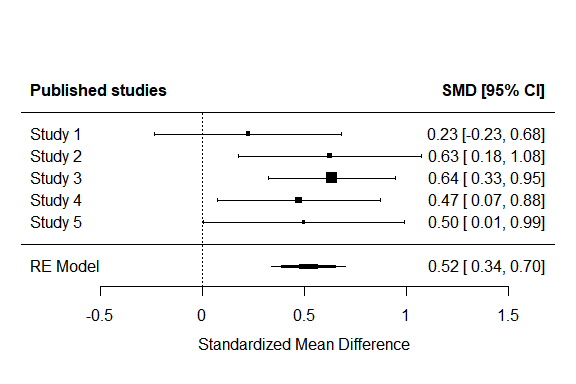
\includegraphics{2_general_structure_of_a_simulation__lesson_files/figure-latex/unnamed-chunk-18-1.pdf}

\hypertarget{wrapping-up}{%
\section{Wrapping up}\label{wrapping-up}}

This lesson taught you about the essential components of a simulation
study, and introduced you to the way in which simulations are actually
built in order to obtain each of those components (i.e., gradually and
with lots of checking along the way).

It then used this simulation to answer a quantitative methods research
question about the statistical power of a Student's \emph{t}-test when
the sample sizes are unbalanced.

To test your learning in this lesson, complete the assignment named
``2\_general\_structure\_of\_a\_simulation\_\_assignment.Rmd''. I will
later pass out a solution to this assignment that you can study and
compare your solution to.

\hypertarget{session-info}{%
\section{Session info}\label{session-info}}

\begin{Shaded}
\begin{Highlighting}[]
\FunctionTok{sessionInfo}\NormalTok{()}
\end{Highlighting}
\end{Shaded}

\begin{verbatim}
## R version 4.3.2 (2023-10-31 ucrt)
## Platform: x86_64-w64-mingw32/x64 (64-bit)
## Running under: Windows 11 x64 (build 22631)
## 
## Matrix products: default
## 
## 
## locale:
## [1] LC_COLLATE=German_Switzerland.utf8  LC_CTYPE=German_Switzerland.utf8   
## [3] LC_MONETARY=German_Switzerland.utf8 LC_NUMERIC=C                       
## [5] LC_TIME=German_Switzerland.utf8    
## 
## time zone: Europe/Zurich
## tzcode source: internal
## 
## attached base packages:
## [1] stats     graphics  grDevices utils     datasets  methods   base     
## 
## other attached packages:
## [1] effsize_0.8.1 ggplot2_3.5.0 purrr_1.0.2   readr_2.1.5   forcats_1.0.0
## [6] dplyr_1.1.4   tidyr_1.3.1  
## 
## loaded via a namespace (and not attached):
##  [1] gtable_0.3.4      highr_0.10        compiler_4.3.2    tidyselect_1.2.0 
##  [5] scales_1.3.0      yaml_2.3.8        fastmap_1.1.1     R6_2.5.1         
##  [9] labeling_0.4.3    generics_0.1.3    knitr_1.45        tibble_3.2.1     
## [13] munsell_0.5.0     pillar_1.9.0      tzdb_0.4.0        rlang_1.1.3      
## [17] utf8_1.2.4        xfun_0.42         viridisLite_0.4.2 cli_3.6.2        
## [21] withr_3.0.0       magrittr_2.0.3    digest_0.6.34     grid_4.3.2       
## [25] rstudioapi_0.15.0 hms_1.1.3         lifecycle_1.0.4   vctrs_0.6.5      
## [29] evaluate_0.23     glue_1.7.0        farver_2.1.1      fansi_1.0.6      
## [33] colorspace_2.1-0  rmarkdown_2.25    tools_4.3.2       pkgconfig_2.0.3  
## [37] htmltools_0.5.7
\end{verbatim}

\end{document}
